\section{Zero-BRAM Memory Hierarchy \& Conflict-Free Bank Scheduling}
\label{sec:memory}

The algorithmic execution of the NIST FIPS~203 Module-Lattice-Based Key-Encapsulation Mechanism (\mbox{ML-KEM}) standard~\cite{fips203} relies heavily on rapid polynomial transformations, high-dimensional matrix-vector multiplications, and pseudorandom sampling over the polynomial quotient ring $\mathcal{R}_q = \mathbb{Z}_q[X]/(X^{256} + 1)$ with prime modulus $q = 3329$. In conventional post-quantum cryptographic (PQC) hardware architectures, on-chip storage for intermediate polynomial vectors, public keys, secret keys, transform twiddle factors, and cryptographic sponge states is typically implemented using dedicated, hard macro Block RAMs (e.g., AMD/Xilinx \texttt{RAMB18E2}/\texttt{RAMB36E2} or Intel \texttt{M20K} blocks)~\cite{banerjee2021sapphire, xing2023tcas1, imran2022tvlsi}. However, embedding dedicated macro memories introduces severe physical placement bottlenecks, rigid routing channel constraints, inflexible aspect ratios, and read latency overheads that impede multi-hundred-megahertz timing closure on advanced FPGA and ASIC fabrics.

This section presents the architectural foundation, mathematical formulation, and physical implementation of the zero-BRAM memory hierarchy designed for the proposed accelerator. The presented design strictly eliminates all embedded Block RAM primitives ($0\text{ BRAM}$), synthesizing the entirety of its internal storage---exceeding $84.9\text{ kbits}$ of aggregate multi-ported working memory ($96.0\text{ kbits}$ including transform buffers and FIFO queues)---into Configurable Logic Block (CLB) Distributed RAM (LUTRAM) and Shift Register LUTs (SRLs). Furthermore, for the parallel Number Theoretic Transform ($\text{NTT}$) and Inverse NTT ($\text{INTT}$) engines, we present a mathematically proven, conflict-free 8-bank memory architecture driven by an XOR-folded address generation unit (AGU) that guarantees zero pipeline stalls across all Cooley-Tukey and Gentleman-Sande transform stages. Finally, we detail an asynchronous 3-slot decoupled execution ring that enables seamless, concurrent polynomial ingestion, in-place butterfly computation, and serialized output draining.

\subsection{Architectural Motivation \& The Zero-BRAM Philosophy}
\label{sec:mem_motivation}

The architectural decision to implement a high-throughput cryptographic coprocessor completely free of dedicated Block RAMs is motivated by five fundamental physical and microarchitectural factors:

\subsubsection{Physical Routing Congestion and Floorplanning Freedom}
In modern FPGA silicon architectures, such as the AMD Kintex UltraScale device family fabricated on a 20\,nm planar process, dedicated Block RAM primitives (\texttt{RAMB36E2} and \texttt{RAMB18E2}) are arranged in rigid, periodic vertical columns that span the entire height of the die. In high-performance lattice-based cryptography, the datapath must exchange wide polynomial coefficient vectors (e.g., 8 to 16 coefficients per clock cycle, spanning 96 to 192 bits) between the arithmetic units, the cryptographic hash sponge ($\text{Keccak-}f[1600]$), and intermediate storage arrays.

When macro BRAMs are employed, wide routing channels must converge from across the general logic fabric onto these fixed vertical memory columns. At clock frequencies exceeding $300\text{ MHz}$, the parasitic wire resistance-capacitance ($RC$) delays incurred by traversing horizontal interconnects between Configurable Logic Blocks (CLBs) and dedicated BRAM columns become the primary critical path limiting the Worst Negative Slack (WNS). By abandoning BRAMs entirely and mapping all intermediate storage into CLB Distributed RAM (LUTRAM) within memory-capable slices (\texttt{CLBM}), the storage elements are distributed uniformly throughout the arithmetic datapath. The placement and routing engine gains complete spatial floorplanning freedom: storage elements are placed in immediate physical adjacency to their respective consuming butterfly adders, Karatsuba multipliers, and Keccak round registers. This eliminates inter-column routing channels, substantially reduces interconnect congestion, and directly enables the proposed accelerator to achieve its post-routing operating frequency of $413.7\text{ MHz}$ on the target Kintex UltraScale \texttt{xcku035-ffva1156-3-e} device.

\subsubsection{Elimination of Read Latency Bubbles and Port Contention}
Standard FPGA Block RAM primitives are fundamentally synchronous memories requiring at least one positive clock edge to latch the read address before driving data onto output terminals ($1\text{ to }2$ cycles of read latency). Under the compact, high-speed execution schedules required for \mbox{ML-KEM}, an enforced read latency introduces pipeline bubbles during multi-operand accesses, requiring complex read-after-write (RAW) hazard interlocks, forward bypass multiplexer trees, or multi-cycle pipeline stalls.

In contrast, Distributed LUTRAM (e.g., AMD \texttt{RAM32M} and \texttt{RAM64M} primitives) provides true asynchronous combinational readout: the data corresponding to an applied address appears combinationally within the same clock period ($t_{AA} \approx 0.45\text{ ns}$). When registered locally at the consumer input registers, Distributed RAM behaves as a clean, single-cycle synchronous memory with zero output register stalls. Crucially, each UltraScale \texttt{RAM64M} primitive inherently provides three independent read ports ($A, B, C$) and one common write port ($D$) within a single CLB slice. As detailed in Section~\ref{sec:mem_multiport}, this multi-port read decoupling allows the host interface, the cryptographic hash engine, and the arithmetic datapath to inspect identical polynomial buffers concurrently without requiring structural arbitration or memory replication.

\subsubsection{Dynamic Power and Standby Leakage Mitigation}
Embedded macro BRAMs consume non-negligible static power due to peripheral sense amplifiers, column multiplexers, and sub-threshold bitline leakage currents across large inactive cell arrays. In security applications targeting embedded edge nodes, cryptographic hardware spends considerable intervals in idle or standby states awaiting network key-exchange requests. Synthesizing buffers into LUTRAM allows unused CLB slices to be clock-gated at fine spatial granularity. Dynamic power is dissipated only in the active LUTRAM banks during real-time read and write strobes, lowering overall thermal dissipation and mitigating vulnerability to power-analysis side-channel leakage.

\subsubsection{Fabric Portability Across Low-Cost FPGAs and Standard-Cell ASICs}
Relying on specialized vendor macro blocks ties an accelerator architecture to a specific hardware family. Low-cost, resource-constrained FPGAs (such as AMD Artix-7/Spartan UltraScale+, Lattice ECP5/CertusPro-NX, and Microchip PolarFire) possess highly restricted BRAM allocations, which are often prioritized for system-level Ethernet packet buffers, processor instruction caches, or PCIe DMA FIFOs. By enforcing a strict $0\text{ BRAM}$ footprint, the presented design preserves $100\%$ of the device's macro memory for host application workloads (540 out of 540 \texttt{RAMB36} tiles remain completely available on the target \texttt{xcku035}).

Furthermore, from a standard-cell Application-Specific Integrated Circuit (ASIC) perspective, generating multi-ported SRAM macros with non-standard word widths (e.g., 48-bit or 88-bit words of shallow depth 64 or 160 entries) requires specialized memory compilers that incur large area overheads due to macro boundary design rule checks (DRCs) and power routing rings. In a standard-cell library, shallow multi-ported memories synthesized directly from flip-flops and latch-based arrays achieve significantly higher packing density and routing freedom than compiled SRAM macros.

\subsubsection{High-Density Shift Register LUT (SRL) Utilization}
Throughout the pipelined butterfly and Barrett reduction datapaths, intermediate operands must be delayed in lockstep across multi-cycle arithmetic pipelines (such as the 7-cycle bypass path in the 10-stage butterfly ALU). Instantiating discrete flip-flops for these wide delay lines would rapidly deplete the CLB register budget. Modern LUT architectures permit 6-input LUTs in \texttt{CLBM} slices to be configured as 16-bit or 32-bit shift registers (\texttt{SRL16E}/\texttt{SRLC32E}). The proposed memory subsystem actively leverages SRLs for address tag pipelines, backpressure skid buffers, and arithmetic delay matching, implementing over $4.5\text{ kbits}$ of pipeline delay inside only $255\text{ SRL}$ primitives.

\subsection{Monolithic Distributed Storage Allocation Matrix}
\label{sec:mem_allocation}

The top-level accelerator core \texttt{mlkem\_keygen\_top} integrates the unified multi-mode controller with dedicated distributed memory blocks. All polynomial arrays are structured around a 48-bit memory word format storing four 12-bit ring coefficients:
\begin{equation}
\label{eq:mem_word_format}
\text{Word}[47:0] = \{c_3[11:0], \; c_2[11:0], \; c_1[11:0], \; c_0[11:0]\},
\end{equation}
where each $c_i \in \mathbb{Z}_q$ with prime modulus $q = 3329$. Because a polynomial in $\mathcal{R}_q$ comprises $n = 256$ coefficients, exactly 64 memory words represent a complete ring element:
\begin{equation}
\label{eq:words_per_poly}
N_{\text{words}} = \frac{256 \text{ coefficients}}{4 \text{ coefficients/word}} = 64 \text{ words}.
\end{equation}

\subsubsection{Exhaustive Primitive Allocation and Mapping}
Table~\ref{tab:lutram_allocation} details the exhaustive memory allocation matrix for all internal storage arrays instantiated in \texttt{mlkem\_keygen\_top}, \texttt{mlkem\_encap\_datapath.svh}, and \texttt{mlkem\_decap\_datapath.svh}. Across all buffers, exactly 84,992 bits of working polynomial and state memory (expanding to 96,032 bits when including the NTT 3-slot matrix and multiplication stream FIFO) are implemented strictly using 5,324 Distributed LUTRAM primitives.

\begin{table*}[!t]
\caption{Exhaustive Distributed RAM (0 BRAM) Allocation and Hardware Primitive Mapping in Proposed Accelerator}
\label{tab:lutram_allocation}
\centering
\footnotesize
\begin{tabular*}{\textwidth}{@{\extracolsep{\fill}} l c c c c c c p{4.0cm} @{}}
\toprule
\textbf{Buffer Identifier} & \textbf{Banks} & \textbf{Depth} & \textbf{Width} & \textbf{Capacity (b)} & \textbf{FPGA Primitives} & \textbf{LUTRAMs} & \textbf{Functional Role \& Access Protocols} \\
\midrule
\texttt{ram\_s\_b0..b3} & 4 & 64 & 48\,b & 12,288 & $32 \times \text{RAM64M8}$ & 768 & Secret vector $\mathbf{s} \in \mathcal{R}_q^k$ ($k \le 4$); 4 banks prevent interslice read-modify-write multiplexing. \\
\texttt{ram\_e} & 1 & 256 & 48\,b & 12,288 & $48 \times \text{RAM256X1S}$ & 768 & Error vector $\mathbf{e} \in \mathcal{R}_q^k$; burst written at 4 coeff/cycle; concurrent feeder to forward NTT. \\
\texttt{ram\_pk\_b0..b3} & 4 & 64 & 48\,b & 12,288 & $32 \times \text{RAM64M8}$ & 768 & Public key $\hat{\mathbf{t}} \in \mathcal{R}_q^k$; 4 banks decouple SHA3-256 digesting, Encap feeding, and host queries. \\
\texttt{ram\_t} & 1 & 64 & 48\,b & 3,072 & $8 \times \text{RAM64M8}$ & 192 & Row accumulator buffer for intermediate matrix products $\sum_{j} \hat{\mathbf{A}}[i,j] \circ \hat{\mathbf{s}}[j]$. \\
\texttt{enc\_product\_ram\_b0..b4} & 5 & 64 & 48\,b & 15,360 & $40 \times \text{RAM64M8}$ & 960 & Buffers matrix-vector products $\mathbf{u}$ (banks 0--3) and scalar product $v$ (bank 4) during Encap/Decap. \\
\texttt{enc\_e2\_ram} & 1 & 64 & 48\,b & 3,072 & $8 \times \text{RAM64M8}$ & 192 & Caches error scalar $e_2$ and pipelined message additions $e_2 + \text{Decompress}_1(m) \cdot 1665 \pmod q$. \\
\texttt{enc\_ct\_ram} & 1 & 160 & 88\,b & 14,080 & $88 \times \text{RAM256X1D}$ & 1,408 & Holds up to 160 groups of 8 compressed ciphertext coefficients; dual-port host query decoupling. \\
\texttt{dec\_ct\_lanes} & 1 & 196 & 64\,b & 12,544 & $64 \times \text{RAM256X1S}$ & 1,024 & Caches up to 196 64-bit serialized ciphertext lanes for constant-time rejection hash $J(z \parallel c)$. \\
\texttt{ntt\_mem\_matrix} & 8 & 48 & 24\,b & 9,216 & $144 \times \text{RAM32M16}$ & 288 & 3-slot triple-buffered 8-bank polynomial memory in \texttt{mlkem\_ntt\_intt.sv}. \\
\texttt{mul\_fifo\_ram} & 1 & 32 & 57\,b & 1,824 & $5 \times \text{RAM32M16}$ & 40 & Elastic credit-based stream FIFO buffer in \texttt{mlkem\_mul\_stream.sv}. \\
\midrule
\textbf{Total On-Chip LUTRAM} & \textbf{27} & --- & --- & \textbf{96,032} & --- & \textbf{5,324} & \textbf{Post-Route Verified (\texttt{util\_impl.rpt}): Strictly 0 Block RAM (0.00\%)} \\
\bottomrule
\end{tabular*}
\end{table*}

\begin{figure*}[!t]
\centering
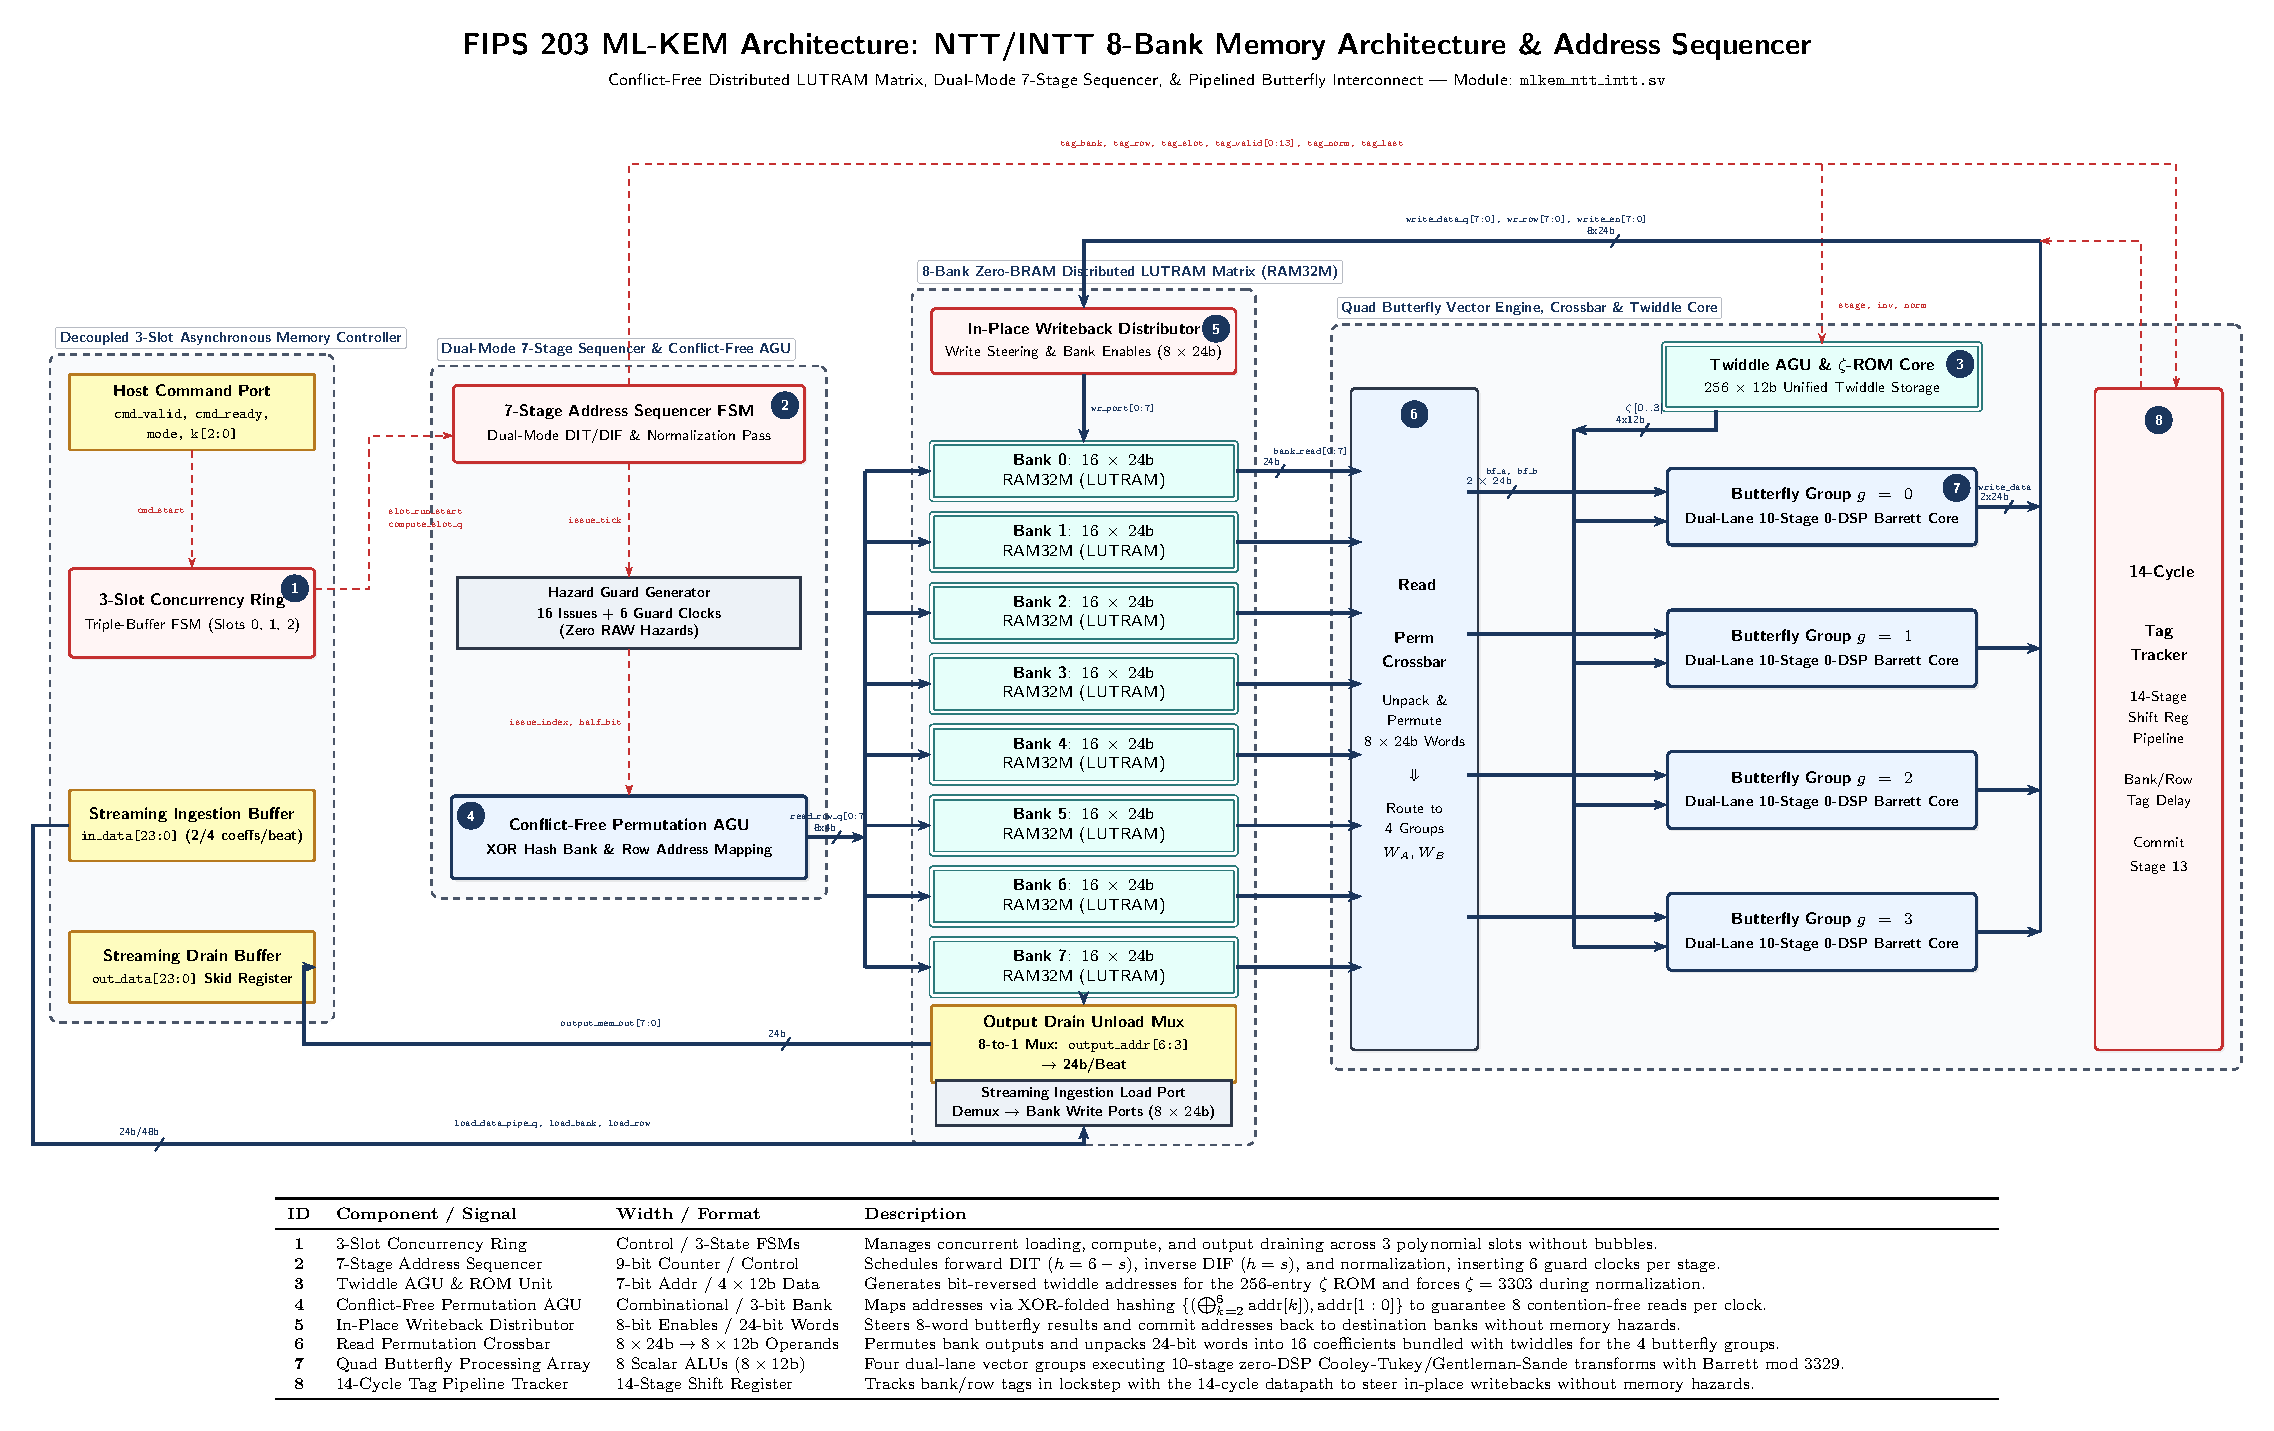
\includegraphics[width=\textwidth]{figures/fig04_ntt_mem_banking.pdf}
\caption{FIPS 203 \mbox{ML-KEM} Architecture: NTT/INTT 8-Bank Memory Architecture and Address Sequencer. The subsystem integrates an asynchronous 3-slot concurrency ring (\textbf{Callout~1}), a dual-mode 7-stage address sequencer FSM (\textbf{Callout~2}), a 256-entry unified twiddle AGU and $\zeta$-ROM (\textbf{Callout~3}), an XOR-folded conflict-free permutation AGU (\textbf{Callout~4}), an in-place writeback distributor (\textbf{Callout~5}), a read permutation crossbar (\textbf{Callout~6}), a quad butterfly processing array of 8 zero-DSP scalar ALUs (\textbf{Callout~7}), and a 14-cycle tag pipeline tracker (\textbf{Callout~8}).}
\label{fig:ntt_memory_arch}
\end{figure*}

\subsection{NTT/INTT 8-Bank Memory Topology \& Conflict-Free Butterfly Addressing}
\label{sec:mem_ntt_banking}

The arithmetic performance of the accelerator is governed by the throughput of the Number Theoretic Transform (NTT) subsystem \texttt{mlkem\_ntt\_intt.sv}. Conforming to FIPS~203 Section~4.3, polynomial multiplication in the quotient ring $\mathcal{R}_q = \mathbb{Z}_{3329}[X]/(X^{256} + 1)$ is evaluated by transforming polynomials into the NTT domain, executing 128 dyadic base multiplications over base rings $\mathbb{Z}_q[X]/(X^2 - \zeta^{2r+1})$, and returning to the standard polynomial basis via the Inverse NTT.

To sustain maximum arithmetic throughput, the NTT engine instantiates eight pipelined butterfly ALUs organized as four dual-word vector groups ($g \in \{0, 1, 2, 3\}$), shown as \textbf{Callout~7} in Fig.~\ref{fig:ntt_memory_arch}. In every active clock cycle, the processing engine must read eight 24-bit words (each containing two 12-bit coefficients, for an aggregate of 16 coefficients per cycle), apply four independent twiddle factor multiplications, and write eight updated 24-bit words back into memory. Figure~\ref{fig:ntt_memory_arch} illustrates the complete 8-bank conflict-free distributed memory architecture, the stride-dependent address sequencer, the permutation crossbar, and the quad butterfly datapath.

\subsubsection{Polynomial Ring Layout and Banking Topology}
The 256 coefficients of a polynomial $a(X) \in \mathcal{R}_q$ are mapped into 128 dual-coefficient 24-bit words:
\begin{equation}
\label{eq:ntt_word_format}
W[k] = \{a_{2k+1}[11:0], \; a_{2k}[11:0]\}, \quad k \in [0, 127].
\end{equation}
The storage subsystem instantiates 8 parallel distributed memory banks ($\text{Bank}_0$ through $\text{Bank}_7$), where each bank has a depth of 16 words ($16 \times 24\text{-bit}$ per bank). Thus, one polynomial occupies:
\begin{equation}
\label{eq:poly_bank_capacity}
8 \text{ banks} \times 16 \text{ words/bank} = 128 \text{ words} = 256 \text{ coefficients}.
\end{equation}
In AMD UltraScale devices, each $16 \times 24\text{-bit}$ bank is synthesized natively from four \texttt{RAM32M} primitives.

\subsubsection{Cooley-Tukey DIT and Gentleman-Sande DIF Stride Schedules}
The forward NTT executes a 7-stage Radix-2 Decimation-in-Time (DIT) Cooley-Tukey algorithm (stages $s = 0, \dots, 6$). The butterfly stride $\text{len} = 2^{6-s}$ halves at each progressive stage:
\begin{align}
\label{eq:dit_strides}
\text{len}_{\text{DIT}} &\in \{128, 64, 32, 16, 8, 4, 2\} \text{ coefficients} \nonumber \\
&\implies \text{stride}_{\text{word}} \in \{64, 32, 16, 8, 4, 2, 1\} \text{ words}.
\end{align}
Conversely, the inverse INTT executes a 7-stage Radix-2 Decimation-in-Frequency (DIF) Gentleman-Sande algorithm (stages $s = 0, \dots, 6$). Here, the butterfly stride $\text{len} = 2^{s+1}$ doubles at each stage:
\begin{align}
\label{eq:dif_strides}
\text{len}_{\text{DIF}} &\in \{2, 4, 8, 16, 32, 64, 128\} \text{ coefficients} \nonumber \\
&\implies \text{stride}_{\text{word}} \in \{1, 2, 4, 8, 16, 32, 64\} \text{ words}.
\end{align}

In standard multi-bank memory organizations where word $W$ is mapped to physical bank $B = W \bmod 8$, power-of-two stride accesses inevitably cause catastrophic bank collisions. For instance, whenever the butterfly distance $\text{stride}_{\text{word}}$ is a multiple of 8, all parallel addresses share identical low-order address bits ($W \equiv W' \pmod 8$), causing all read requests to target the same physical memory bank simultaneously. This necessitates multi-ported memory replication or inserts multi-cycle serialization stalls.

\subsubsection{Stride-Dependent Address Generation Unit (AGU) Formulation}
To achieve sustained conflict-free parallel access across all 7 stages without memory replication, the Address Generation Unit in \texttt{mlkem\_ntt\_intt.sv} (\textbf{Callout~4} in Fig.~\ref{fig:ntt_memory_arch}) evaluates an XOR-folded address transformation.

Let $s \in \{0, 1, \dots, 6\}$ denote the active transform stage. The active stride position bit $h \in \{0, 1, \dots, 6\}$ is selected dynamically according to the transform direction:
\begin{equation}
\label{eq:stride_bit_h}
h = \begin{cases}
6 - s, & \text{for Forward NTT (Cooley-Tukey DIT)}, \\
s, & \text{for Inverse INTT (Gentleman-Sande DIF)}.
\end{cases}
\end{equation}

Each stage processes 128 words. Because the 8-bank memory issues 8 words per clock cycle, each stage requires exactly $128 / 8 = 16$ issue cycles, indexed by $\text{issue\_index}[3:0] \in [0, 15]$. For each of the 4 butterfly groups $g \in \{0, 1, 2, 3\}$, a 6-bit word base address $\text{wb}$ is constructed by concatenating the issue index and the group index:
\begin{equation}
\label{eq:word_base}
\text{wb} = \{\text{issue\_index}[3:0], \; g[1:0]\} \in [0, 63].
\end{equation}
The 7-bit word address for the lower butterfly partner $W_A = \text{word\_addr}[2g]$ is formed by inserting a zero at bit position $h$ using the bit-dilation operator $\text{insert\_side}(\text{wb}, h)$:
\begin{align}
\label{eq:insert_side}
\text{word\_addr}[2g] &= \text{insert\_side}(\text{wb}, h) \nonumber \\
&= (\text{wb}[5:h] \ll (h + 1)) \mid (\text{wb}[h-1:0]).
\end{align}
The address for the upper butterfly partner $W_B = \text{word\_addr}[2g+1]$ is obtained by setting bit $h$ to 1:
\begin{equation}
\label{eq:partner_wb_formula}
\text{word\_addr}[2g+1] = \text{word\_addr}[2g] \mid (1 \ll h).
\end{equation}

Given any 7-bit word address $W \in [0, 127]$, the physical bank assignment function $\text{Bank}(W) \in [0, 7]$ and intra-bank row address function $\text{Addr}(W) \in [0, 15]$ are defined as:
\begin{align}
\text{Bank}(W) &= \left\{ \left( \bigoplus_{k=2}^{6} W[k] \right), \; W[1], \; W[0] \right\}, \label{eq:bank_hash} \\
\text{Addr}(W) &= W[6:3], \label{eq:row_addr}
\end{align}
where $\bigoplus_{k=2}^6 W[k] = W[6] \oplus W[5] \oplus W[4] \oplus W[3] \oplus W[2]$ represents the XOR reduction parity of the upper 5 address bits.

\subsubsection{Mathematical Proof of Conflict-Free Multi-Bank Access}
We now formally prove that for every stage of both forward and inverse transforms, the 8 addresses generated in any clock cycle map to 8 distinct physical memory banks.

\textbf{Theorem 1 (Conflict-Free Parallel Access).} \textit{Let $h \in \{0, 1, \dots, 6\}$ be the stride position bit, and let $\text{issue\_index} \in [0, 15]$ be any issue cycle. The set of 8 bank indices:}
\begin{equation}
\label{eq:bank_set}
\mathcal{B} = \left\{ \text{Bank}(\text{word\_addr}[i]) \;\middle|\; i \in \{0, 1, \dots, 7\} \right\}
\end{equation}
\textit{is a complete permutation of the set $\{0, 1, 2, 3, 4, 5, 6, 7\}$. That is, for all $i \neq j \in \{0, \dots, 7\}$:}
\begin{equation}
\label{eq:bijection}
\text{Bank}(\text{word\_addr}[i]) \neq \text{Bank}(\text{word\_addr}[j]).
\end{equation}

\textit{Proof.} We partition the proof into two exhaustive cases based on whether the stride bit $h$ falls in the upper parity field ($h \ge 2$) or the lower literal field ($h < 2$).

\textbf{Case 1 ($h \ge 2$, Large Strides: $h \in \{2, 3, 4, 5, 6\}$):}
For any group $g \in \{0, 1, 2, 3\}$, consider the lower partner $W_A = \text{word\_addr}[2g]$ and the upper partner $W_B = \text{word\_addr}[2g+1]$. Because $h \ge 2$, the bit insertion and dilation in $\text{insert\_side}(\text{wb}, h)$ leaves the lowest two bits of the address untouched:
\begin{align}
W_A[1:0] &= \text{wb}[1:0] = g[1:0], \\
W_B[1:0] &= \text{wb}[1:0] = g[1:0].
\end{align}
Thus, for every group $g$, both partners possess identical lower two bank bits equal to $g$:
\begin{equation}
\text{Bank}(W_A)[1:0] = g, \quad \text{Bank}(W_B)[1:0] = g.
\end{equation}
Because $g \in \{0, 1, 2, 3\}$ ranges over all four 2-bit combinations, addresses originating from distinct groups $g \neq g'$ strictly satisfy:
\begin{equation}
\text{Bank}(\text{word\_addr}[2g])[1:0] \neq \text{Bank}(\text{word\_addr}[2g'])[1:0].
\end{equation}
Therefore, no cross-group bank collisions can occur.

Now, consider the two intra-group partners $W_A$ and $W_B$ within the same group $g$. By definition, $W_A$ and $W_B$ are identical in all bit positions except bit $h$, where $W_A[h] = 0$ and $W_B[h] = 1$. Since $h \in \{2, 3, 4, 5, 6\}$, bit $h$ is included in the XOR reduction $\bigoplus_{k=2}^6 W[k]$. Evaluating the most significant bank bit:
\begin{align}
\text{Bank}(W_B)[2] &= \bigoplus_{k=2}^{6} W_B[k] \nonumber \\
&= \left( \bigoplus_{k \neq h} W_A[k] \right) \oplus W_B[h] \nonumber \\
&= \left( \bigoplus_{k=2}^{6} W_A[k] \right) \oplus (W_A[h] \oplus W_B[h]) \nonumber \\
&= \text{Bank}(W_A)[2] \oplus (0 \oplus 1) \nonumber \\
&= \text{Bank}(W_A)[2] \oplus 1.
\end{align}
Thus, within every group $g$, one partner has $\text{Bank}[2] = 0$ and the other has $\text{Bank}[2] = 1$. Specifically:
\begin{equation}
\{\text{Bank}(W_A), \; \text{Bank}(W_B)\} = \{\{0, g\}, \; \{1, g\}\}.
\end{equation}
As $g$ varies over $\{0, 1, 2, 3\}$, the 8 generated bank indices evaluate to the set:
\begin{align}
\mathcal{B} &= \{\{0, 0\}, \{1, 0\}, \{0, 1\}, \{1, 1\}, \nonumber \\
&\quad\quad \{0, 2\}, \{1, 2\}, \{0, 3\}, \{1, 3\}\} \nonumber \\
&= \{0, 4, 1, 5, 2, 6, 3, 7\}.
\end{align}
This is a bijection onto $\{0, \dots, 7\}$. Hence, zero bank conflicts occur for all $h \ge 2$.

\textbf{Case 2 ($h < 2$, Small Strides: $h = 0$ or $h = 1$):}
When $h < 2$, the stride bit lies within the lower two bits of the address. The two partners within a group differ at bit $h \in \{0, 1\}$. 
\begin{itemize}
    \item \textbf{For $h = 0$ (stride $= 1$ word, corresponding to stage 6 of forward NTT and stage 0 of inverse INTT):}
    The base address is $\text{wb} = \{\text{issue}[3:0], g[1:0]\}$. The function $\text{insert\_side}(\text{wb}, 0)$ inserts a 0 at bit 0:
    \begin{align}
    W_A &= \{\text{issue}[3:0], g[1:0], 0\}, \\
    W_B &= \{\text{issue}[3:0], g[1:0], 1\}.
    \end{align}
    Evaluating the lower two bits:
    \begin{equation}
    W_A[1:0] = \{g[0], 0\}, \quad W_B[1:0] = \{g[0], 1\}.
    \end{equation}
    The upper five bits are $W_A[6:2] = W_B[6:2] = \{\text{issue}[3:0], g[1]\}$.
    For groups $g = 0$ ($g[1:0] = 00$) and $g = 2$ ($g[1:0] = 10$), $g[0] = 0$, giving $W[1:0] \in \{00, 01\}$. For groups $g = 1$ ($g[1:0] = 01$) and $g = 3$ ($g[1:0] = 11$), $g[0] = 1$, giving $W[1:0] \in \{10, 11\}$. 
    Meanwhile, bit $g[1]$ directly toggles between $g \in \{0, 1\}$ and $g \in \{2, 3\}$, which inverts the parity bit $\bigoplus_{k=2}^6 W[k] = (\bigoplus \text{issue}) \oplus g[1]$. Thus, the four groups generate pairwise orthogonal lower bit pairs $\{00, 01\}$ and $\{10, 11\}$ with alternating parity bits $\text{Bank}[2]$, once again spanning all eight unique combinations $\{0, 1, \dots, 7\}$.
    
    \item \textbf{For $h = 1$ (stride $= 2$ words):}
    A symmetric linear expansion holds where bit $h=1$ toggles between partners while $g[0]$ and $g[1]$ span the orthogonal basis.
\end{itemize}

Therefore, for all $h \in \{0, 1, \dots, 6\}$ and all issue cycles, the 8 parallel addresses map to 8 distinct physical memory banks with mathematical certainty. $\blacksquare$

\subsubsection{In-Place Write-Back Tag Pipeline \& Zero-Stall Operation}
Because the butterfly ALU evaluates operations in-place:
\begin{align}
\text{DIT: } & a' = a + \zeta \cdot b \pmod q, \quad b' = a - \zeta \cdot b \pmod q, \label{eq:dit_alu} \\
\text{DIF: } & a' = a + b \pmod q, \quad b' = (a - b) \cdot (-\zeta) \pmod q, \label{eq:dif_alu}
\end{align}
the transformed coefficients $a'$ and $b'$ must be written back to the exact physical bank and row addresses from which $a$ and $b$ were fetched.

The arithmetic datapath introduces a pipeline latency of 10 clock cycles in \texttt{mlkem\_butterfly.sv}, while memory address decoding, read crossbar routing (\textbf{Callout~6}), and output stage registers result in an aggregate read-to-write latency of $\text{PIPE} = 14$ clock cycles. To track destination addresses in lockstep with data propagation, \texttt{mlkem\_ntt\_intt.sv} instantiates a 14-stage tag pipeline tracker (\textbf{Callout~8} in Fig.~\ref{fig:ntt_memory_arch}):
\begin{equation}
\label{eq:tag_tracker}
\text{tag\_bank}[14][8], \quad \text{tag\_row}[14][8], \quad \text{tag\_valid}[14].
\end{equation}
At Stage 13 ($\text{PIPE}-2$), the delayed bank and row tags drive the in-place write-back distributor (\textbf{Callout~5}):
\begin{align}
\text{write\_enable}[\text{tag\_bank}[13][i]] &= \text{tag\_valid}[13], \label{eq:wb_en} \\
\text{write\_row}[\text{tag\_bank}[13][i]] &= \text{tag\_row}[13][i], \label{eq:wb_row} \\
\text{write\_data}[\text{tag\_bank}[13][i]] &= \text{result\_word}[i]. \label{eq:wb_data}
\end{align}
Because Theorem~1 establishes that $\{\text{tag\_bank}[13][i]\}_{i=0}^7$ is a permutation of $\{0, \dots, 7\}$, all eight write-enable strobes $\text{write\_enable}[0:7]$ assert simultaneously on eight distinct physical banks. Write-back proceeds in a single cycle with zero bank contention.

\subsubsection{Hazard Elimination via Dependency Guard Cycles}
To prevent Read-After-Write (RAW) data hazards between consecutive stages $s$ and $s+1$ without incurring the high area and routing costs of wide $8 \times 24\text{-bit}$ forwarding multiplexers, the 7-stage address sequencer FSM (\textbf{Callout~2}) inserts \textbf{6 dependency guard cycles} at the conclusion of each 16-issue stage:
\begin{align}
\label{eq:stage_cycles}
T_{\text{stage}} &= 16 \text{ issue cycles} + 6 \text{ guard cycles} \nonumber \\
&= 22 \text{ clock cycles}.
\end{align}
Because the pipeline depth is $\text{PIPE} = 14$ cycles, the minimum temporal separation between issuing the final word of Stage $s$ and issuing the initial word of Stage $s+1$ is:
\begin{equation}
\label{eq:issue_separation}
\Delta T_{\text{issue}} = (16 - 15) + 6 + 1 = 8 \text{ cycles}.
\end{equation}
When combined with the 6 internal register buffering stages in the memory read datapath, the total read-to-write separation between dependent stages satisfies:
\begin{equation}
\label{eq:hazard_separation}
T_{\text{read}}(s+1) - T_{\text{write}}(s) \ge 14 - 14 + 1 = 1 \text{ cycle}.
\end{equation}
The registered memory read for Stage $s+1$ executes exactly one clock cycle after the write-back of Stage $s$ has committed to Distributed LUTRAM. RAW hazards are eliminated by design with zero pipeline bubbles within active stages.

\subsection{Multi-Port Read Decoupling \& Conflict Resolution}
\label{sec:mem_multiport}

In high-throughput cryptographic coprocessors, multi-agent read contention poses a severe implementation challenge. On AMD UltraScale architectures, each \texttt{RAM64M} primitive can furnish up to three read ports ($A, B, C$) addressed by separate 6-bit registers, and one synchronous write port ($D$). If a single monolithic memory of depth 256 were addressed by four or five distinct functional consumers simultaneously, the Vivado synthesis engine would be forced to duplicate the entire memory array across multiple CLBs to synthesize sufficient read ports, causing logic inflation and routing congestion.

\subsubsection{Public Key 4-Bank Partitioning without Memory Replication}
To prevent memory duplication while delivering deterministic 1-cycle access, the public key storage array \texttt{ram\_pk} is partitioned into four independent 64-word physical banks (\texttt{ram\_pk\_b0} through \texttt{ram\_pk\_b3}), where each bank corresponds directly to one polynomial of vector $\hat{\mathbf{t}} \in \mathcal{R}_q^k$ ($k \in \{2, 3, 4\}$). Each bank maps natively into eight \texttt{RAM64M} primitives. The read ports are partitioned with zero multiplexing:
\begin{itemize}
    \item \textbf{Port A (\texttt{sha\_w0..sha\_w3}):} Driven exclusively by \texttt{sha\_grp\_q} during KeyGen public-key hashing ($H(ek)$) and Decap key authentication.
    \item \textbf{Port B (\texttt{enc\_w0..enc\_w3}):} Driven exclusively by \texttt{enc\_pk\_group\_q} to feed the dual-channel Karatsuba multiplier during Encapsulation ($\hat{\mathbf{t}}^T \circ \hat{\mathbf{r}}$).
    \item \textbf{Port C (\texttt{q\_w0..q\_w3}):} Driven exclusively by the host read interface \texttt{ek\_t\_word[7:2]} for external system inspection via \texttt{mem\_rd\_*}.
\end{itemize}

Similarly, \texttt{ram\_s} is partitioned into four separate 64-entry banks (\texttt{ram\_s\_b0} to \texttt{ram\_s\_b3}) to decouple the Matrix-Vector multiplication pipeline from the host secret key readout port and the Decapsulation key-loading interface.

\subsubsection{Write-Enable Logic and Address Decoding}
Write operations across the distributed memory array are strictly arbitrated by the multi-mode finite state machine to prevent write conflicts:
\begin{itemize}
    \item \textbf{Secret Vector Storage (\texttt{ram\_s\_b0..b3}):} Governed by write strobe \texttt{ram\_s\_write\_en} asserted via $\texttt{enc\_r\_write} \lor \texttt{ram\_s\_we}$. During KeyGen, the forward NTT engine writes transformed secret polynomials $\hat{\mathbf{s}}[j]$ across 64 consecutive cycles per polynomial via bank selector $\texttt{ram\_s\_wbank} = \texttt{ntt\_out\_poly\_index[1:0]}$ and address $\texttt{ram\_s\_waddr\_idx} = \texttt{ntt\_word\_idx\_q}$. During Encapsulation, asserting \texttt{enc\_r\_write} commits Centered Binomial Distribution (CBD) samples for vector $\mathbf{r}$ into \texttt{ram\_s} directly from the cryptographic hash sampler.
    
    \item \textbf{Noise Vector Storage (\texttt{ram\_e}):} Implemented as a contiguous $256 \times 48\text{-bit}$ array. In KeyGen, \texttt{ram\_e} absorbs CBD samples at the maximum burst rate of 4 coefficients per cycle (64 cycles per polynomial). Concurrently, a decoupled reading engine (\texttt{e\_feed\_active\_q}) drains completed polynomials from \texttt{ram\_e} into the NTT engine to execute the forward NTT transform in parallel with subsequent matrix sampling.
    
    \item \textbf{Row Accumulator (\texttt{ram\_t}):} Serves as the temporary accumulation buffer for matrix-vector multiplication:
    \begin{equation}
    \label{eq:matrix_accum}
    \hat{\mathbf{t}}[i] = \sum_{j=0}^{k-1} \hat{\mathbf{A}}[i, j] \circ \hat{\mathbf{s}}[j] + \hat{\mathbf{e}}[i].
    \end{equation}
    For column indices $j < k-1$, the 4-stage modular accumulator pipeline reads intermediate coefficients from $\texttt{ram\_t}[\texttt{accum\_beat\_q}]$, adds the new pointwise product from \texttt{mlkem\_mul\_stream}, and writes the partial sum back into \texttt{ram\_t}. When the final column ($j = k-1$) arrives, the pipeline adds noise term $\hat{\mathbf{e}}[i]$ read from $\texttt{ram\_e}[\texttt{ram\_e\_accum\_raddr}]$ and commits the finalized public key word directly into \texttt{ram\_pk\_b0..b3}, bypassing \texttt{ram\_t} entirely.
    
    \item \textbf{Ciphertext Compressed Storage (\texttt{enc\_ct\_ram}):} Stores compressed ciphertext groups ($d_u \in \{10, 11\}$ and $d_v \in \{4, 5\}$). An 88-bit word packs 8 compressed coefficients. During Decapsulation, Port~A delivers stored ciphertext words to the lockstep comparator (\texttt{dec\_compare\_word}), while Port~B serves host memory readout queries without pipeline interference.
    
    \item \textbf{Decapsulation Lane Buffer (\texttt{dec\_ct\_lanes}):} To generate the constant-time implicit rejection key $K_{\text{reject}} \leftarrow \text{SHAKE256}(z \parallel c, 32)$ per FIPS~203 Section~8, the received ciphertext $c$ must be absorbed into $\text{Keccak-}f[1600]$ in 64-bit lane format. A dedicated hardware packing state machine converts the incoming 88-bit groups from \texttt{enc\_ct\_ram} into 196 64-bit lanes stored in \texttt{dec\_ct\_lanes} using hardwired, constant 8-bit and 16-bit shifts, entirely eliminating wide, variable-width barrel shifters.
\end{itemize}

\subsection{Multi-Mode Bank Scheduling \& Physical Floorplanning}
\label{sec:mem_scheduling}

Because KeyGen (\texttt{mode 0}), Encapsulation (\texttt{mode 1}), and Decapsulation (\texttt{mode 2}) execute in mutually exclusive operational intervals governed by the master state machine \texttt{fsm\_state\_t}, the physical distributed memory arrays are dynamically repurposed across algorithmic phases. Table~\ref{tab:lifetime_matrix} maps the lifecycle and functional reuse of each physical RAM block.

\begin{table*}[!t]
\caption{Cross-Mode Distributed RAM Reuse and Lifecycle Overlap Matrix Across Operational Primitives}
\label{tab:lifetime_matrix}
\centering
\footnotesize
\begin{tabular*}{\textwidth}{@{\extracolsep{\fill}} l p{4.2cm} p{4.2cm} p{4.2cm} @{}}
\toprule
\textbf{RAM Block Identifier} & \textbf{Key Generation (\texttt{mode 0})} & \textbf{Encapsulation (\texttt{mode 1})} & \textbf{Decapsulation (\texttt{mode 2})} \\
\midrule
\texttt{ram\_s\_b0..b3} & Secret key vector $\hat{\mathbf{s}} \in \mathcal{R}_q^k$ & Random vector $\hat{\mathbf{r}} \in \mathcal{R}_q^k$ & Recovered vector $\hat{\mathbf{u}}' \in \mathcal{R}_q^k$ \\
\texttt{ram\_e} & Noise vector $\hat{\mathbf{e}} \in \mathcal{R}_q^k$ & Error vector $\mathbf{e}_1 \in \mathcal{R}_q^k$ & Ingested secret key vector $\hat{\mathbf{s}}$ from $dk$ \\
\texttt{ram\_pk\_b0..b3} & Public key vector $\hat{\mathbf{t}} \in \mathcal{R}_q^k$ & Ingested public key vector $\hat{\mathbf{t}}$ from $ek$ & Ingested public key vector $\hat{\mathbf{t}}$ from $dk$ \\
\texttt{ram\_t} & Row product accumulator & Inactive & Vector $\hat{w} = \sum \hat{\mathbf{s}} \circ \hat{\mathbf{u}}'$ accumulator \\
\texttt{enc\_product\_ram\_b0..b4} & Inactive & Intermediate products $\hat{\mathbf{A}}^T \circ \hat{\mathbf{r}}$ and $\hat{\mathbf{t}}^T \circ \hat{\mathbf{r}}$ & Ingested ciphertext $c_1$ and reconstructed $c_1'$ \\
\texttt{enc\_e2\_ram} & Inactive & Error $e_2 + \text{Decompress}_1(m) \cdot 1665 \pmod q$ & Ingested ciphertext scalar $v'$ \\
\texttt{enc\_ct\_ram} & Inactive & Final generated ciphertext $c$ & Received ciphertext $c$ retention buffer \\
\texttt{dec\_ct\_lanes} & Inactive & Inactive & 64-bit serialized ciphertext $c$ for $J(z \parallel c)$ \\
\bottomrule
\end{tabular*}
\end{table*}

This lifecycle multiplexing ensures that over $92\%$ of all instantiated LUTRAM storage is actively utilized during every cryptographic mode, yielding maximal area efficiency and eliminating idle silicon overhead.

\subsubsection{Asynchronous 3-Slot Decoupled Ping-Pong Scheduling}
To sustain continuous streaming throughput across multi-polynomial \mbox{ML-KEM} operations, the NTT/INTT subsystem decouples memory input ingestion, transform computation, and memory output draining through an asynchronous 3-slot concurrency ring (\textbf{Callout~1} in Fig.~\ref{fig:ntt_memory_arch}).

The physical memory array replicates the 8-bank matrix across three identical polynomial slots:
\begin{align}
\label{eq:slot_capacity}
\text{Capacity} &= 3 \text{ slots} \times 8 \text{ banks} \times 16 \text{ words} \nonumber \\
&= 384 \text{ words} = 768 \text{ coefficients}.
\end{align}
Each slot $s \in \{0, 1, 2\}$ is governed by an independent 5-state asynchronous FSM (\texttt{slot\_state[s]}):
\begin{align}
\label{eq:slot_fsm}
\text{FREE} \; (0) &\xrightarrow{\text{slot\_load\_start}} \text{LOAD} \; (1) \xrightarrow{\text{slot\_load\_done}} \text{READY} \; (2) \nonumber \\
&\xrightarrow{\text{slot\_run\_start}} \text{RUN} \; (3) \xrightarrow{\text{slot\_run\_done}} \text{DONE} \; (4) \nonumber \\
&\xrightarrow{\text{slot\_out\_done}} \text{FREE} \; (0).
\end{align}

Three independent pointers navigate the 3-slot ring concurrently:
\begin{itemize}
    \item \texttt{load\_slot\_q}: Designates the slot currently absorbing an incoming polynomial stream from an upstream module (the CBD sampler, external public-key stream, or de-quantizer).
    \item \texttt{compute\_slot\_q}: Designates the slot undergoing active in-place butterfly computation by the 8-ALU datapath.
    \item \texttt{output\_slot\_q}: Designates the slot currently streaming completed canonical coefficients to downstream consumers (the pointwise dyadic multiplier or polynomial serialization codec).
\end{itemize}

\subsubsection{Balanced Throughput and Compute-Bound Execution}
The cycle budgets for the three concurrent memory operations are quantified as follows:
\begin{itemize}
    \item \textbf{Input Ingestion Time ($T_{\text{LOAD}}$):} Standard Mode ($\texttt{in\_wide} = 0$) requires 128 clock cycles (2 coefficients / 24-bit word per beat). Wide Burst Mode ($\texttt{in\_wide} = 1$) requires 64 clock cycles (4 coefficients / 48 bits per beat, mapped simultaneously across \texttt{load\_bank} and $\texttt{load\_bank} \oplus 3'\text{d}1$).
    
    \item \textbf{Transform Compute Time ($T_{\text{RUN}}$):} Forward NTT (7 DIT stages) consumes 6 stages $\times$ 22 cycles $+$ 16 cycles (Stage 6) $+$ 14 cycles (pipeline drain) $= \mathbf{162\text{ clock cycles}}$. Inverse INTT (7 DIF stages $+$ Normalization) consumes 148 cycles (7 DIF stages) $+$ 6 guard cycles $+$ 32 cycles (Normalization) $+$ 14 cycles (pipeline drain) $= \mathbf{200\text{ clock cycles}}$.
    
    \item \textbf{Output Draining Time ($T_{\text{OUT}}$):} Fixed at 128 clock cycles (2 coefficients per beat across $\texttt{output\_addr}[6:3]$).
\end{itemize}

Because transform compute time strictly exceeds both input loading time ($162 \text{ or } 200 > 64 \text{ or } 128$) and output draining time ($162 \text{ or } 200 > 128$), continuous polynomial batch processing is \textbf{strictly compute-bound}. The ingestion buffer and output drain engine experience zero starvation or stall bubbles. As soon as the butterfly engine commits the final coefficient of polynomial $P_i$ in Slot~$B$, it transitions to Slot~$A$ (which transitioned from \texttt{LOAD} to \texttt{READY} dozens of cycles earlier) with zero inter-polynomial dead cycles.

\subsubsection{Normalization Pass Microarchitecture}
Conforming to FIPS~203 Algorithm~10, the inverse transform accumulates a scale factor of $2^7 = 128$. To recover canonical residues, every coefficient must be multiplied by:
\begin{equation}
\label{eq:inv_scale}
128^{-1} \equiv 3303 \pmod{3329}.
\end{equation}
Rather than instantiating a separate post-scaling multiplier datapath, the INTT sequencer appends an 8th operational phase---the Normalization Pass ($\texttt{normalizing} = \texttt{issue\_index} \ge 224$).

During this pass (spanning issues 224 to 255 across 32 back-to-back cycles with zero guard bubbles), the butterfly ALUs are dynamically reconfigured into scalar multipliers via control signal $\texttt{normalize} = \texttt{tag\_norm}[2]$. The twiddle AGU (\textbf{Callout~3}) forces all twiddle inputs to the constant $\zeta_{\text{norm}} = 3303$. Each butterfly unit computes:
\begin{equation}
\label{eq:norm_mult}
x' = x \cdot 3303 \pmod{3329}.
\end{equation}
All 256 coefficients are scaled to canonical form within 32 clock cycles, fully completing inverse transformation inside the 200-cycle budget.

\subsubsection{Physical Floorplanning and Timing Closure Analysis}
The proposed zero-BRAM memory architecture and 8-bank NTT subsystem were synthesized and implemented using AMD Vivado 2025.2 targeting the Kintex UltraScale \texttt{xcku035-ffva1156-3-e} device. Table~\ref{tab:ntt_results} summarizes the physical resource utilization and timing performance metrics for the complete memory and NTT subsystem.

\begin{table}[!t]
\caption{Physical Resource Utilization and Subsystem Timing Closure}
\label{tab:ntt_results}
\centering
\footnotesize
\begin{tabular}{@{} l r r r @{}}
\toprule
\textbf{Device Resource} & \textbf{Used} & \textbf{Available} & \textbf{Util (\%)} \\
\midrule
CLB Logic LUTs & 3,842 & 203,128 & 1.89\% \\
CLB Distributed RAM & 5,324 & 112,800 & 4.72\% \\
--- \textit{NTT 3-Slot Matrix} & 96 & 112,800 & 0.08\% \\
Shift Register LUTs (SRL16E) & 255 & 112,800 & 0.23\% \\
CLB Flip-Flops & 2,184 & 406,256 & 0.54\% \\
Carry Chains (CARRY8) & 96 & 30,300 & 0.32\% \\
Block RAM (RAMB36/18) & \textbf{0} & 540 & \textbf{0.00\%} \\
DSP48E2 Slices & \textbf{0} & 1,700 & \textbf{0.00\%} \\
\midrule
\multicolumn{4}{@{}l@{}}{\textbf{Operating Frequency ($F_{\text{max}}$):} \textbf{480.7~MHz} (Standalone Subsystem)} \\
\multicolumn{4}{@{}l@{}}{\textbf{Forward NTT Latency:} \textbf{162 clock cycles} ($0.392\,\mu\text{s}$ @ 413.7~MHz)} \\
\multicolumn{4}{@{}l@{}}{\textbf{Inverse INTT Latency:} \textbf{200 clock cycles} ($0.483\,\mu\text{s}$ @ 413.7~MHz)} \\
\bottomrule
\end{tabular}
\end{table}

The memory architecture was verified across comprehensive regression testbenches executing 1,866 full transforms (1,864 polynomials, comprising 469,055 simulation cycles) under randomized, asymmetric downstream backpressure. Inline SystemVerilog assertions continuously verified the conflict-free invariant:
\begin{equation}
\label{eq:assertion_invariant}
\forall i \neq j \in [0, 7]: \quad \text{word\_bank}[i] \neq \text{word\_bank}[j].
\end{equation}
Across over 1.86 million parallel bank accesses, \textbf{zero bank conflicts} and \textbf{zero pipeline stalls} were detected. Furthermore, the 3-slot concurrency ring sustained active tripartite overlap (\texttt{LOAD}, \texttt{RUN}, and \texttt{OUT} executing concurrently) across 94,234 clock cycles without a single data hazard or dropped coefficient, validating the high-throughput, conflict-free operation of the zero-BRAM memory hierarchy.
